\documentclass[final]{beamer}

\usetheme{enziteto}

\usepackage[orientation=portrait, size=a0, scale=1.4, debug]{beamerposter}
\usepackage{booktabs}
\usepackage{dcolumn}
\usepackage{colortbl}
\usepackage{xcolor}
\usepackage{hyperref}
\usepackage{amsmath}
\usepackage[absolute,overlay,showboxes]{textpos}
\usepackage{calc}
\usepackage[colorgrid,texcoord]{eso-pic}
% \usepackage[style=authoryear-comp, backref=true]{biblatex}

\usepackage{blindtext}


% \usepackage{xparse}
% \ExplSyntaxOn
% \NewDocumentCommand{\convertto}{mm}
% % #1 = em or ex (or any other unit)
% % #2 = dimen to convert
% {
%   \texttt{#2~=~\fp_to_decimal:n { round ( #2/1#1, 5 ) }#1}
% }
% \DeclareExpandableDocumentCommand{\thelength}{ O{mm} m }
% {
%   \fp_to_decimal:n { round ( #2/1#1, 5 ) } #1
% }
% \ExplSyntaxOff


%
% debugging colors
\definecolor{header}{RGB}{200, 125, 25}
\definecolor{footer}{RGB}{0, 153, 51}

\setbeamertemplate{itemize item}{\raisebox{.21ex}{\hbox{\tiny\textcolor{lacamlilac}{$\boldsymbol{\oplus}$}}\hspace{-2pt}}}
\setbeamertemplate{itemize subitem}{\raise .2ex\hbox{\tiny\textcolor{lacamlilac}{$\boldsymbol{\otimes}$}}\hspace{-3pt}}
\setbeamertemplate{itemize subsubitem}{\textcolor{lacamlilac}{$\oplus$}}
\setbeamertemplate{bibliography item}{\hspace{10pt}\raise .2ex\hbox{\tiny\textcolor{lacamlilac}{$\boldsymbol{\oplus}$}}}


% \setbeamertemplate{headline}{}

% \addbibresource{../referomnia/referomnia.bib}

\title{Simplifying, Regularizing and Strengthening Sum-Product Network Structure Learning}
\author{Antonio  Vergari, Nicola  {Di Mauro} and Floriana Esposito}
\date{}


\begin{document}

\institute{Università degli Studi di Bari}
\department{Dipartimento di Informatica}
\laboratory{LACAM}
\group{Machine Learning}
\institutelogo{
\includegraphics[width=25pt]{figures/unibaba}}
\lablogo{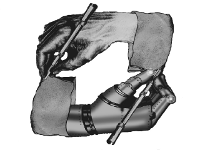
\includegraphics[width=35pt]{figures/lacam}}


% {
%   \setbeamertemplate{headline}{}
%   \setbeamertemplate{footline}{}
%   \begin{textblock}
%     \titlepage
%   \end{textblock}
% }

\newcommand{\hmargin}{20mm}
\newcommand{\vmargin}{20mm}
\textblockorigin{\hmargin}{\vmargin}

\setlength{\TPHorizModule}{1cm}
\setlength{\TPVertModule}{1cm}

%
% TODO: generalize this
\newlength{\posterwidth}
\setlength{\posterwidth}{841mm - 2\hmargin}
\newlength{\posterheight}
\setlength{\posterheight}{1189mm}

\newcommand{\ncols}{3}
\newlength{\colwidth}
\setlength{\colwidth}{\posterwidth/\ncols}


\newlength{\colhpoint}


\begin{frame}{}
  %
  % title
  % \textblockcolour{header}
  \begin{textblock}{58}(0, 0)
    \usebeamerfont{section name}
    \huge
    Simplifying, Regularizing and Strengthening\\
    Sum-Product Network Structure Learning
  \end{textblock}
  %
  % authors
  \begin{textblock}{30}(0, 6.5)
    \usebeamerfont{author}
    \small
    Antonio  Vergari, Nicola  {Di Mauro} and Floriana Esposito
  \end{textblock}
  % 
  % email
  \begin{textblock}{15}(30, 6.5)
    \usebeamerfont{author}
    \small
    \emph{\{firstname.lastname@uniba.it\}}
  \end{textblock}
  %
  % affiliations
  \begin{textblock}{20}(60, 0)
    \usebeamerfont{author}
    \scriptsize
    \begin{minipage}[t]{5cm}
      \vspace{0pt}\hspace{10pt}
      
\includegraphics[width=90pt]{figures/unibaba}
    \end{minipage}
    \begin{minipage}[t]{12cm}
    \vspace{27pt}
      \flushleft
      University of Bari "Aldo Moro", Italy\\
    \vspace{2pt}
      Department of Computer Science
    \end{minipage}\\[0.75cm]
    \usebeamerfont{author}
    \scriptsize
    \begin{minipage}[t]{5cm}
      \vspace{0pt}
      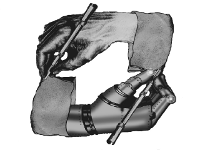
\includegraphics[width=110pt]{figures/lacam}
    \end{minipage}
    \begin{minipage}[t]{12cm}
      \vspace{23pt}
      \flushleft
      LACAM\\
      \vspace{2pt}
      Machine Learning
    \end{minipage}
  \end{textblock}
  
  
  %
  % section 1
  \begin{textblock}{80}(0, 9.8)
    \usebeamerfont{section name}
    Sum-Product Networks and Tractable Models
  \end{textblock}
  
  
  \begin{textblock}{25.7}(0, 12.3)
    \small
    Tractable inference on Probabilistic Graphical Models (PGMs) is
    at a trade off with model expressiveness.
    \begin{table}[!ht]
      \setlength{\tabcolsep}{35pt}
      \centering
      \begin{tabular}{c c}
        
        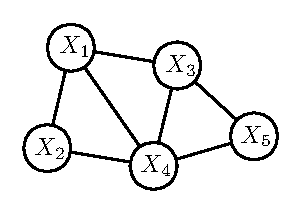
\includegraphics[width=0.25\linewidth]{figures/mrf} &
                                                              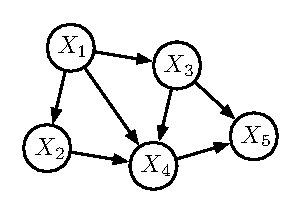
\includegraphics[width=0.25\linewidth]{figures/bn}\\
        \addlinespace[-0.2cm]
        \scriptsize  $P(\mathbf{X})=\frac{1}{Z}\prod_{c}\phi_{c}(\mathbf{X}_{c})$
                                                            & 
                                                              \scriptsize
                                                              $P(\mathbf{X})=\prod_{i=1}^nP(X_{i}|\mathbf{Pa}_{i})$\\
        \addlinespace[0.5cm]
        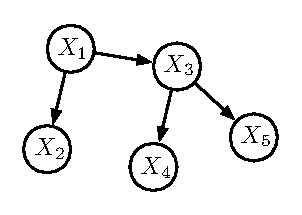
\includegraphics[width=0.25\linewidth]{figures/clt} &
                                                              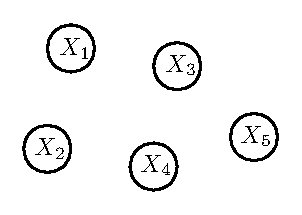
\includegraphics[width=0.25\linewidth]{figures/nf}\\
        \addlinespace[-0.2cm]
        \scriptsize
        $P(\mathbf{X})=\prod_{i=1}^nP(X_{i}|Pa_{i})$ &
                                                       \scriptsize $P(\mathbf{X})=\prod_{i=1}^nP(X_{i})$                                                              
      \end{tabular}
    \end{table}
    
  \end{textblock}
  
  \begin{textblock}{25.7}(27.1, 12.3)
    \small
    \emph{Compiling} the partition function of a pdf into a \textbf{\emph{deep}} architecture of \textbf{sum}
    and \textbf{product} nodes.\\
    
    Product nodes define factorizations over independent vars, sum
    nodes mixtures. Leaves are tractable univariate distributions.\\
    
    % Sum node children weights are the parameters of the model.\\
    
    Products over nodes with different scopes (\emph{decomposability}) and
    sums over nodes with same scopes (\emph{completeness}) guarantee modeling
    a pdf (\emph{validity}).\\
    
    Considering only valid SPNs of \emph{alternated layers of sum and
      products}.
    
    \begin{minipage}{0.45\linewidth}
      \centering
      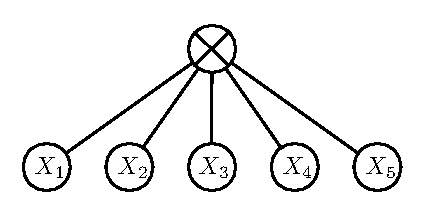
\includegraphics[width=0.8\linewidth]{figures/spn-prod}
    \end{minipage}\begin{minipage}{0.45\linewidth}
      \centering
      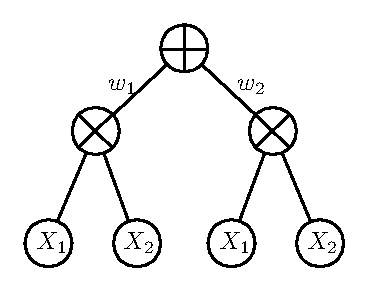
\includegraphics[width=0.7\linewidth]{figures/spn-sum}
    \end{minipage}
    
    
  \end{textblock}
  
  \begin{textblock}{25.7}(54.2, 12.3)
    \small
    \emph{Compiling} the partition function of a pdf into a \textbf{\emph{deep}} architecture of \textbf{sum}
    and \textbf{product} nodes.\\
    
    Product nodes define factorizations over independent vars, sum
    nodes mixtures. Leaves are tractable univariate distributions.\\
    
    % Sum node children weights are the parameters of the model.\\
    
    Products over nodes with different scopes (\emph{decomposability}) and
    sums over nodes with same scopes (\emph{completeness}) guarantee modeling
    a pdf (\emph{validity}).\\
    
    Considering only valid SPNs of \emph{alternated layers of sum and
      products}.
    
    \begin{minipage}{0.45\linewidth}
      \centering
      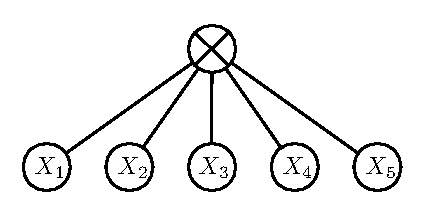
\includegraphics[width=0.8\linewidth]{figures/spn-prod}
    \end{minipage}\begin{minipage}{0.45\linewidth}
      \centering
      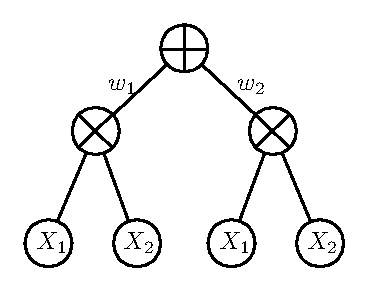
\includegraphics[width=0.7\linewidth]{figures/spn-sum}
x    \end{minipage}


  \end{textblock}
  
  %
  % section 2
  \begin{textblock}{80}(0, 28.5)
    \usebeamerfont{section name}
    How and Why to perform Structure Learning
    
  \end{textblock}
  
  \begin{textblock}{25.7}(0, 31.)
    \small
    \blindtext
  \end{textblock}
  
  \begin{textblock}{25.7}(27.1, 31.)
    \small
    \blindtext
  \end{textblock}
  
  \begin{textblock}{25.7}(54.2, 31.)
    \small
    \blindtext
  \end{textblock}
  
  
  %
  % section 3
  \begin{textblock}{80}(0, 47.2)
    \usebeamerfont{section name}
    Simplifying by Limiting Node Splits
  \end{textblock}
  
  \begin{textblock}{25.7}(0, 49.7)
    \small
    \blindtext
  \end{textblock}
  
  \begin{textblock}{25.7}(27.1, 49.7)
    \small
    \blindtext
  \end{textblock}
  
  \begin{textblock}{25.7}(54.2, 49.7)
    \small
    \blindtext
  \end{textblock}
  
  
  % 
  % section 4
  \begin{textblock}{80}(0, 65.9)
    \usebeamerfont{section name}
    Regularizing by introducing tree distributions as leaves
  \end{textblock}
  
  \begin{textblock}{25.7}(0, 68.4)
    \small
    \blindtext
  \end{textblock}
  
  \begin{textblock}{25.7}(27.1, 68.4)
    \small
    \blindtext
  \end{textblock}
  
  \begin{textblock}{25.7}(54.2, 68.4)
    \small
    \blindtext
  \end{textblock}
  
  
  
  % 
  % section 5
  \begin{textblock}{80}(0, 84.6)
    \usebeamerfont{section name}
    Strengthening by Model Averaging
  \end{textblock}
  
  \begin{textblock}{25.7}(0, 87.1)
    \small
    \blindtext
  \end{textblock}
  
  \begin{textblock}{25.7}(27.1, 87.1)
    \small
    \blindtext
  \end{textblock}
  
  \begin{textblock}{25.7}(54.2, 87.1)
    \small
    \blindtext
  \end{textblock}
  
  
  
  % 
  % section 5
  \begin{textblock}{80}(0, 103.3)
    \usebeamerfont{section name}
    References
  \end{textblock}
  
  \begin{textblock}{25.7}(0, 105.8)
    \small
    % \blindtext
  \end{textblock}
  
  \begin{textblock}{25.7}(27.1, 105.8)
    \small
    % \blindtext
  \end{textblock}
  
  \begin{textblock}{25.7}(54.2, 105.8)
    \small
    % \blindtext
  \end{textblock}

  % 
  % footer
  \begin{textblock}{80}(0, 114.3)
    \usebeamerfont{subtitle}
    \textbf{ECML-PKDD 2015} - 8th September 2015, Porto, Portugal\hfill
    {\url{http://www.di.uniba.it/~vergari/code/spyn.html}}
  \end{textblock}
  
\end{frame}




\end{document}

%%% Local Variables:
%%% mode: latex
%%% TeX-master: t
%%% TeX-engine: xetex
%%% End:
